\documentclass{standalone}
\usepackage[usenames,dvipsnames]{xcolor}
\usepackage{tikz, ifthen}
\usetikzlibrary{arrows.meta}
\usetikzlibrary{positioning}


\begin{document}



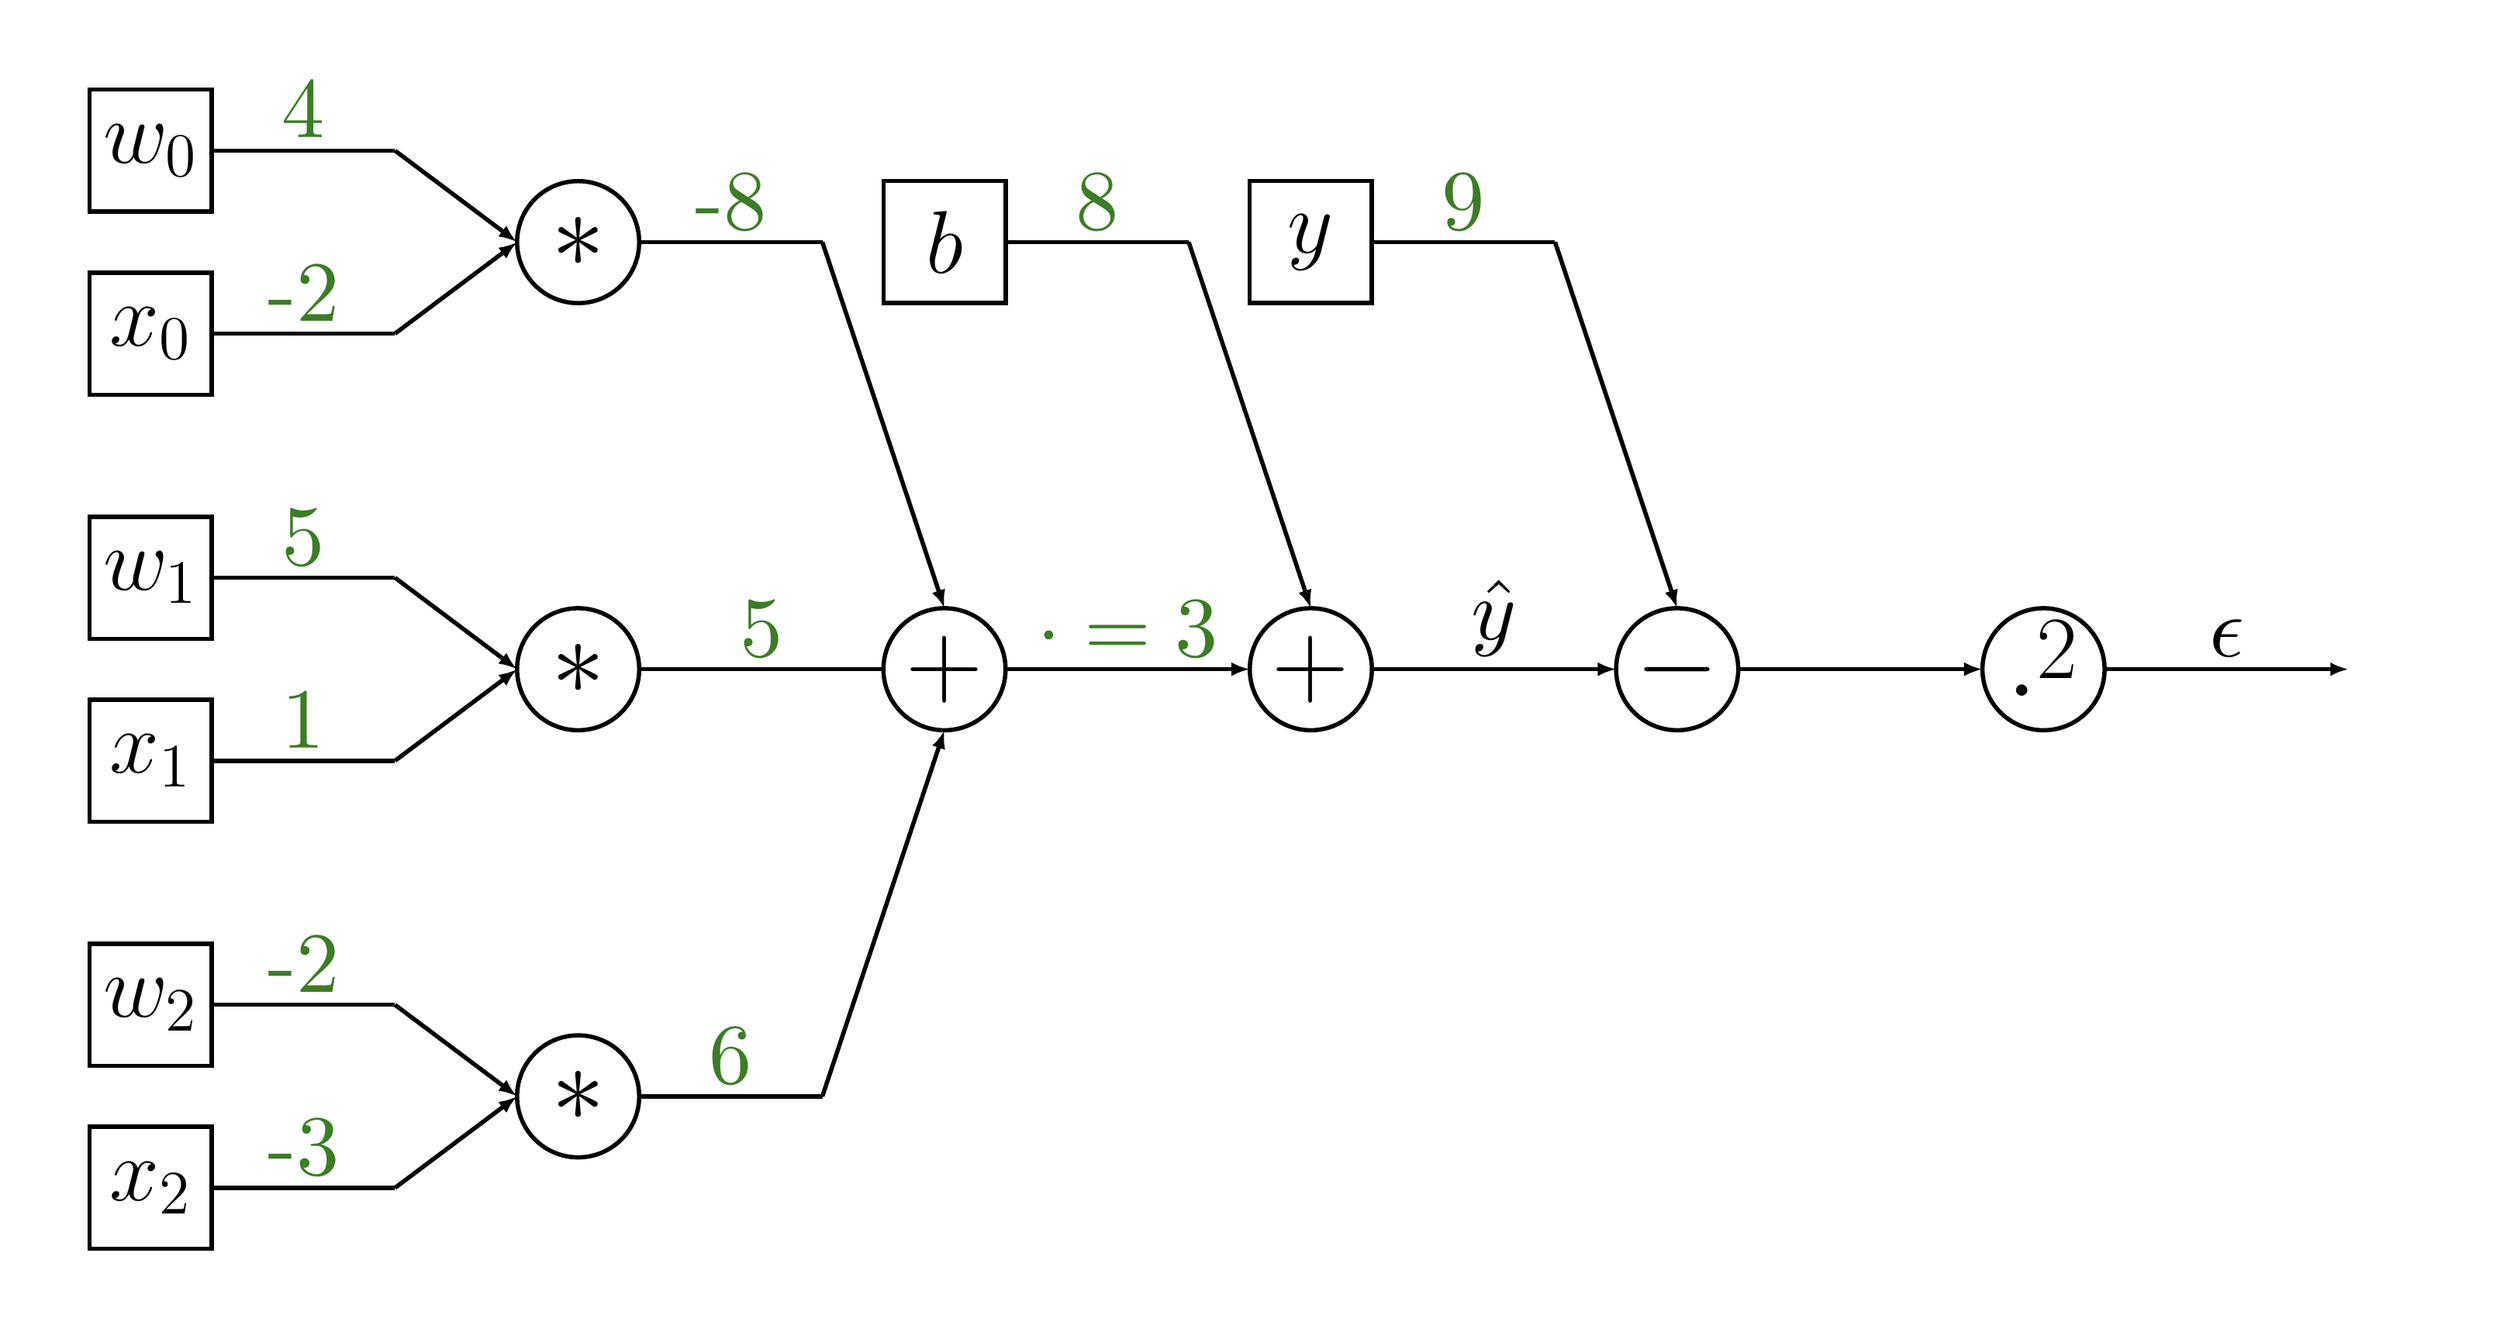
\begin{tikzpicture}[line width=0.7mm]


	
% anchor points for size
\node at (0,-1) {} { };
\node at (40,20) {} { };

% w0
\draw (1,19) rectangle (3, 17);
\node[scale=2] at (2,18) {\huge $w_0$};

% x0
\draw (1,16) rectangle (3,14);
\node[scale=2] at (2,15) {\huge $x_0$};

% op w0 * x0
\draw (9, 16.5) circle (1cm);
\node[scale=2] at (9, 16.5) {\Huge $*$}; 

% arrow from w0 to *
\def\x{3}
\def\y{18}
\def\forward{4}
\def\backward{-8}
\draw (\x, \y) --
%  node[above, shift={(1, -0.4)}, scale=3] {$\textcolor{OliveGreen}{\forward}-\alpha(\textcolor{BrickRed}{\backward})$}
  node[above, shift={(0,-0.4)}, scale=4,text=OliveGreen] {\forward}
%  node[below,shift={(0,0.4)},scale=3,text=BrickRed] {$\frac{\partial\epsilon}{\partial w_0}$}
%  node[below,shift={(0,0.4)},scale=3,text=BrickRed] {$\frac{\partial\epsilon}{\partial w_0}=\backward$}
%  node[below,shift={(0,0.4)},scale=4,text=BrickRed] {\backward}
(\x+3,\y);
\draw [-{Latex[length=3mm]}] (6,18) -- (8,16.5);

% Calculation for gradient of w0
%\node[scale=3.5, align=center] at (21, 4) {$f(w_0, x_0)=w_0 * x_0$ \\ 
%                                           $\frac{\partial f}{\partial w_0}=x_0 = -2$};

% arrow from x0 to *
\def\x{3}
\def\y{15}
\def\forward{-2}
\def\backward{16}
\draw (\x, \y) --
  node[above, shift={(0,-0.4)}, scale=4,text=OliveGreen] {\forward}
%  node[below,shift={(0,0.4)},scale=4,text=BrickRed] {\backward}
(\x+3,\y);
\draw [-{Latex[length=3mm]}] (6,15) -- (8,16.5);

% Calculation for gradient of x0
%\node[scale=3.5, align=center] at (21, 4) {$f(w_0, x_0)=w_0 * x_0$ \\ 
%                                           $\frac{\partial f}{\partial x_0}=w_0 = 4$};

	
% w1
\draw (1,12) rectangle (3,10);
\node[scale=2] at (2,11) {\huge $w_1$};

% x1
\draw (1,9) rectangle (3,7);
\node[scale=2] at (2,8) {\huge $x_1$};

% op w1 * x1
\draw (9, 9.5) circle (1cm);
\node[scale=2] at (9, 9.5) {\Huge $*$}; 

% arrow from w1 to *
\def\x{3}
\def\y{11}
\def\forward{5}
\def\backward{4}
\draw (\x, \y) --
%  node[above, shift={(1, -0.4)}, scale=3] {$\textcolor{OliveGreen}{\forward}-\alpha(\textcolor{BrickRed}{\backward})$}
  node[above, shift={(0,-0.4)}, scale=4,text=OliveGreen] {\forward}
%  node[below,shift={(0,0.4)},scale=3,text=BrickRed] {$\frac{\partial\epsilon}{\partial w_1}$}
%  node[below,shift={(0,0.4)},scale=4,text=BrickRed] {\backward}
(\x+3,\y);
\draw [-{Latex[length=3mm]}] (6,11) -- (8,9.5);


% arrow from x1 to *
\def\x{3}
\def\y{8}
\def\forward{1}
\def\backward{20}
\draw (\x, \y) --
  node[above, shift={(0,-0.4)}, scale=4,text=OliveGreen] {\forward}
%  node[below,shift={(0,0.4)},scale=4,text=BrickRed] {\backward}
(\x+3,\y);
\draw [-{Latex[length=3mm]}] (6,8) -- (8,9.5);

% w2
\draw (1,5) rectangle (3,3);
\node[scale=2] at (2,4) {\huge $w_2$};

% x2
\draw (1,2) rectangle (3,0) ;
\node[scale=2] at (2,1) {\huge $x_2$};

% op w2 * x2
\draw (9, 2.5) circle (1cm);
\node[scale=2] at (9, 2.5) {\Huge $*$}; 

% arrow from w2 to *
\def\x{3}
\def\y{4}
\def\forward{-2}
\def\backward{-12}
\draw (\x, \y) --
%  node[above, shift={(1.5, -0.4)}, scale=3] {$\textcolor{OliveGreen}{\forward}-\alpha(\textcolor{BrickRed}{\backward})$}
  node[above, shift={(0,-0.4)}, scale=4,text=OliveGreen] {\forward}
%  node[below,shift={(0,0.4)},scale=3,text=BrickRed] {$\frac{\partial\epsilon}{\partial w_2}$}
%  node[below,shift={(0,0.4)},scale=4,text=BrickRed] {\backward}
(\x+3,\y);
\draw [-{Latex[length=3mm]}] (6,4) -- (8,2.5);


% arrow from x2 to *
\def\x{3}
\def\y{1}
\def\forward{-3}
\def\backward{-8}
\draw (\x, \y) --
  node[above, shift={(0,-0.4)}, scale=4,text=OliveGreen] {\forward}
%  node[below,shift={(0,0.4)},scale=4,text=BrickRed] {\backward}
(\x+3,\y);
\draw [-{Latex[length=3mm]}] (6,1) -- (8,2.5);


% op sum(w_i * x_i)
\draw (15, 9.5) circle (1cm);
\node[scale=2] at (15, 9.5) {\Huge $+$};

% arrow from w0*x0 to sum
\def\x{10}
\def\y{16.5}
\def\forward{-8}
\def\backward{4}
\draw (\x, \y) --
  node[above, shift={(0,-0.4)}, scale=4,text=OliveGreen] {\forward}
%  node[below,shift={(0,0.4)},scale=4,text=BrickRed] {\backward}
%  node[below,shift={(0,0.4)},scale=4,text=BrickRed] {$\epsilon'=\backward$}
(\x+3,\y);
\draw [-{Latex[length=3mm]}] (13,16.5) -- (15,10.5);



% arrow from w1*x1 to sum
\def\x{10}
\def\y{9.5}
\def\forward{5}
\def\backward{4}
\draw (\x, \y) --
  node[above, shift={(0,-0.4)}, scale=4,text=OliveGreen] {\forward}
%  node[below,shift={(0,0.4)},scale=4,text=BrickRed] {\backward}
(\x+4,\y);


% arrow from w2*x2 to sum
\def\x{10}
\def\y{2.5}
\def\forward{6}
\def\backward{4}
\draw (\x, \y) --
  node[above, shift={(0,-0.4)}, scale=4,text=OliveGreen] {\forward}
%  node[below,shift={(0,0.4)},scale=4,text=BrickRed] {\backward}
(\x+3,\y);
\draw [-{Latex[length=3mm]}] (13,2.5) -- (15,8.5);


% op plus b

% b
\draw (14,17.5) rectangle (16,15.5);
\node[scale=2] at (15,16.5) {\huge $b$};

% arrow from b to +b
\def\x{16}
\def\y{16.5}
\def\forward{8}
\def\backward{4}
\draw (\x, \y) --
%  node[above, shift={(0.5, -0.4)}, scale=3] {$\textcolor{OliveGreen}{\forward}-\alpha(\textcolor{BrickRed}{\backward})$}
  node[above, shift={(0,-0.4)}, scale=4,text=OliveGreen] {\forward}
%  node[below,shift={(0,0.4)},scale=3,text=BrickRed] {$\frac{\partial\epsilon}{\partial b}=4$}
%  node[below,shift={(0,0.4)},scale=4,text=BrickRed] {\backward}
(\x+3,\y);
\draw [-{Latex[length=3mm]}] (19,16.5) -- (21,10.5);

% plus b
\draw (21, 9.5) circle (1cm);
\node[scale=2] at (21, 9.5) {\Huge $+$};

% arrow from sum to +b
\draw [-{Latex[length=3mm]}] (16, 9.5) -- (20,9.5);
\draw [-{Latex[length=3mm]}] (16, 9.5) -- 
  node[above,scale=4,shift={(0,-0.1)},text=OliveGreen] {$\cdot=3$} 
%  node[below,scale=4,shift={(0,0.1)},text=BrickRed] {$4$} 
%  node[below,scale=4,shift={(0,0.1)},text=BrickRed] {$\epsilon'=4$} 
(20,9.5);

% arrow from +b to -y
\draw [-{Latex[length=3mm]}] (22, 9.5) -- (26,9.5);
\draw [-{Latex[length=3mm]}] (22, 9.5) -- 
  node[above, shift={(0,-0.4)},scale=4] {$\hat{y}$}
%  node[above, shift={(0,-0.4)},text=OliveGreen,scale=4] {$\hat{y}=11$}
%  node[below,scale=4,shift={(0,0.1)},text=BrickRed] {$4$} 
%  node[below,scale=4,shift={(0,0.1)},text=BrickRed] {$\epsilon'=4$} 
(26,9.5);
%\draw [-{Latex[length=3mm]}] (22, 9.5) -- node[above,scale=4,text=OliveGreen] {$\hat{y}=11$} node[below,scale=4,text=BrickRed] {4} (26,9.5);

%\node[scale=3.5, align=center] at (21, 4) {$f(\cdot, b)=\cdot + b$ \\ 
%                                           $\frac{\partial f}{\partial b}=1$};



%% y
\draw (20,17.5) rectangle (22,15.5);
\node[scale=2] at (21,16.5) {\huge $y$};

% arrow from y to -y
\draw (22,16.5) -- (25,16.5);
\draw (22,16.5) -- 
  node[above,scale=4,shift={(0,-0.1)},text=OliveGreen] {9} 
%  node[below,scale=4,shift={(0,0.1)},text=BrickRed] {$-4$} 
(25,16.5);
\draw [-{Latex[length=3mm]}] (25,16.5) -- (27,10.5);

%\node[scale=3.5, align=center] at (28, 4) {$f(y, \hat{y})=y-\hat{y}$ \\ 
%                                           $\frac{\partial f}{\partial \hat{y}}=-1$};



% minus y
\draw (27, 9.5) circle (1cm);
\node[scale=2] at (27, 9.5) {\Huge $-$};


% ^2
\draw (33, 9.5) circle (1cm);
\node[scale=2] at (33, 9.5) {\Huge $\cdot^2$};

% arrow from -y to square
\draw [-{Latex[length=3mm]}] (28, 9.5) -- (32,9.5);
\draw [-{Latex[length=3mm]}] (28, 9.5) -- 
%  node[above,scale=3.5,shift={(0,-0.1)},text=OliveGreen] {$\Delta=-2$} 
%  node[below,scale=3.7,text=BrickRed,shift={(0,0.1)}] {$-4$}
%  node[below,scale=3.7,text=BrickRed,shift={(0,0.1)}] {$\epsilon'=-4$}
%  node[below,scale=3,text=BrickRed,shift={(0,0.1)}] {$\frac{d\epsilon}{d\Delta}=-4$}
(32,9.5);



%\node[scale=3.5, align=center] at (33, 4) {$f(\Delta)=\Delta^2$ \\ 
%                                         $\frac{df}{d\Delta}=2\Delta=-4$ \\
%                                         $\frac{d\epsilon}{d\Delta} = \frac{df}{d\Delta}\cdot\epsilon' = -4\cdot1$};

% arrow out of square
\draw [-{Latex[length=3mm]}] (34, 9.5) -- 
  node[above,scale=4,shift={(0,-0.1)}] {$\epsilon$}
%  node[above,scale=4,text=OliveGreen,shift={(0,-0.1)}] {$\epsilon=4$} 
%  node[below,scale=4,text=BrickRed,shift={(0,0.1)}] {1}
%  node[below,scale=4,text=BrickRed,shift={(0,0.1)}] {$\epsilon'=1$}
%  node[below,scale=4,text=BrickRed,shift={(0,0.1)}] {$\frac{d\epsilon}{d\epsilon}=1$}
(38,9.5);



\end{tikzpicture}

\end{document}